\documentclass{beamer}

\usepackage{listings}
\usepackage[color]{circus}
\usepackage{tikz}
\usepackage{amsthm}
\usepackage{algorithmicx}
\usepackage{algpseudocode}
\usepackage{algorithm}

\lstset{language=C}

\usetikzlibrary{calc}

\tikzset{onslide/.code args={<#1>#2}{\only<#1>{\pgfkeysalso{#2}}}}

\newtheorem{rul}{Rule}

% \useoutertheme{miniframes}

\title{Algebraic Compilation\\of Safety-Critical Java Bytecode}
\author{James Baxter}
\date{Thesis Seminar\\19 March 2018}

\begin{document}

\frame{\titlepage}

\section{Introduction}
\stepcounter{subsection}

\begin{frame}
  \frametitle{Motivation}
  \begin{itemize}
  \item Java for real-time and embedded systems
  \item Safety-Critical Java (SCJ)
  \item Differences from standard Java
    \begin{itemize}
    \item Scheduling
    \item Memory management
    \item No dynamic class loading
    \end{itemize}
  \item Requires a specialised SCJ virtual machine (SCJVM)
  \item Existing SCJVMs:~icecap HVM, Fiji VM, OVM
    \begin{itemize}
    \item Compilation for efficiency
    \item No formal verification
    \item icecap:~the only publicly-available up-to-date SCJVM
    \end{itemize}
  \end{itemize}
\end{frame}

\begin{frame}
  \frametitle{Contributions}
  \begin{itemize}
  \item Formal model of an SCJVM interpreter
  \item Compilation strategy
    \begin{itemize}
    \item Acts on Java bytecode in the interpreter
    \item Outputs a shallow embedding of C code
    \item Specification of how to apply compilation rules
    \end{itemize}
  \item Compilation rules
    \begin{itemize}
    \item Provable formal rules
    \item Act on the interpreter model
    \end{itemize}
  \end{itemize}
\end{frame}

\section{Preliminaries}
\stepcounter{subsection}

\begin{frame}
  \frametitle{Safety-Critical Java}
  \begin{itemize}
  \item An SCJ program is made up of missions, which are executed sequentially, in an order determined by a \texttt{MissionSequencer}.
  \item A class implementing the \texttt{Safelet} interface initialises the program and supplies the \texttt{MissionSequencer}.
  \item Each mission is made up of event handlers of various types.
  \item Memory is allocated in memory areas with different lifetimes.
  \item Annotations allow for checking that dangling references cannot occur.
  \end{itemize}
  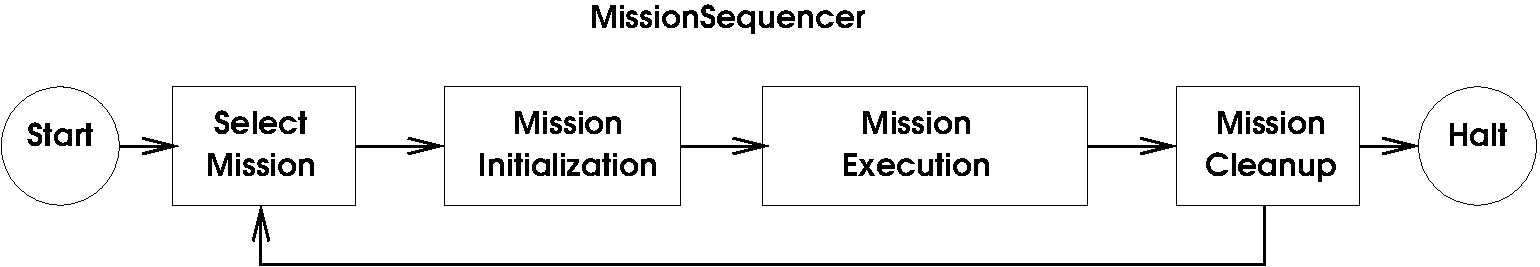
\includegraphics[width=\textwidth]{phases.pdf}
\end{frame}

% \begin{frame}
%   \frametitle{Safety-Critical Java}
%   \begin{columns}
%     \begin{column}{.5\textwidth}
%       \begin{itemize}
%       \item Memory is allocated in memory areas with different lifetimes:
%         \begin{itemize}
%         \item immortal memory
%         \item mission memory
%         \item per-release memory
%         \item temporary private memory
%         \end{itemize}
%       \item Annotations allow for checking that dangling references cannot occur.
%       \end{itemize}
%     \end{column}
%     \begin{column}{.5\textwidth}
%       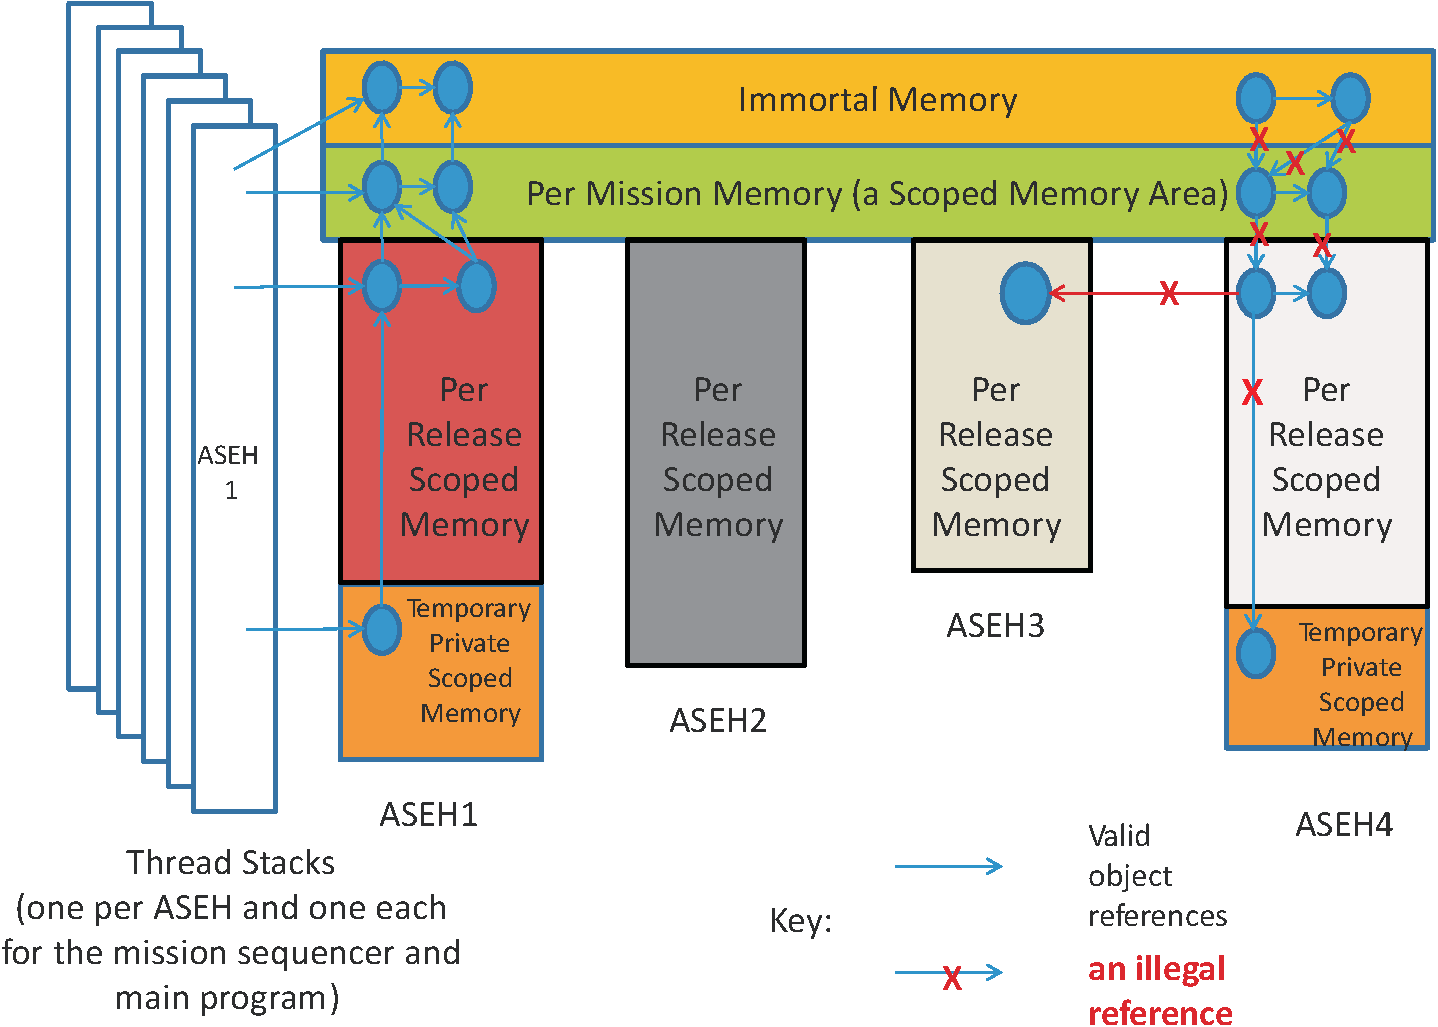
\includegraphics[width=\textwidth]{../../pictures/Stacks-Areas.pdf}
%     \end{column}
%   \end{columns}
% \end{frame}

\begin{frame}
  \frametitle{\Circus{}}
  \begin{itemize}
  \item Based on CSP and the Z notation
  \item CSP to specify processes that communicate over channels
  \item Z to specify state and data operations
  \item \Circus{} specifications are made up of processes with encapsulated
    state that may be made up of multiple actions.
  \item Channels represent the interface of a process.
  \item Processes may be composed in parallel.
  \item Notation for refinement
  \end{itemize}
  
  \begin{columns}[c]
    \tiny
    \setlength{\zedindent}{0cm}
    \setlength{\zedleftsep}{0.1cm}
    \setlength{\zedtab}{0.5cm}
    \column{0.5\textwidth}
  \begin{circus}
    \circchannel getInstruction : ProgramAddress \\
    \circchannel getInstructionRet : Bytecode \\
  \end{circus}
  \vspace{-1.3cm}
  \begin{circus}
    \t2 \vdots
  \end{circus}
  \vspace{-1cm}
  \begin{circus}
    \circprocess Interpreter \circdef \circbegin
  \end{circus}
  \vspace{-1cm}
  \begin{schema}{InterpreterState}
    frameStack : \seq StackFrame \\
    pc : ProgramAddress \\
    currentClass : Class
  \where
    % definition of currentClass (only important if the frame stack is nonempty)
  frameStack \neq \emptyset \implies \\
  \t1 currentClass = \\
  \t2 (last~frameStack).frameClass
  \end{schema}
  \vspace{-1cm}
  \begin{circusaction}
    \circstate InterpreterState
  \end{circusaction}
  \vfill
  \column{0.5\textwidth}
  \vspace{-0.5cm}
  \begin{schema}{InterpreterInit}
    InterpreterState~'
  \where
    frameStack' = \emptyset
  \end{schema}
  \vspace{-1cm}
  \begin{circusaction}
    \t2\vdots
  \end{circusaction}
  \vspace{-1cm}
  \begin{circusaction}
    Loop \circdef \\
    \t1 (frameStack \neq \emptyset) \circguard HandleInstruction \\
    \t1 {} \extchoice (frameStack = \emptyset) \circguard StartInterpreter \circseq \\
    \t1 Loop
  \end{circusaction}
  \vspace{-0.8cm}
  \begin{circusaction}
    \circspot \lschexpract InterpreterInit \rschexpract \circseq Loop
  \end{circusaction}
  \vspace{-1cm}
  \begin{circus}
    \circend
  \end{circus}
  \vfill
\end{columns}
\end{frame}
  
\section{Interpreter Model}
\stepcounter{subsection}

\begin{frame}
  \frametitle{Overview of Model}
  \centering
  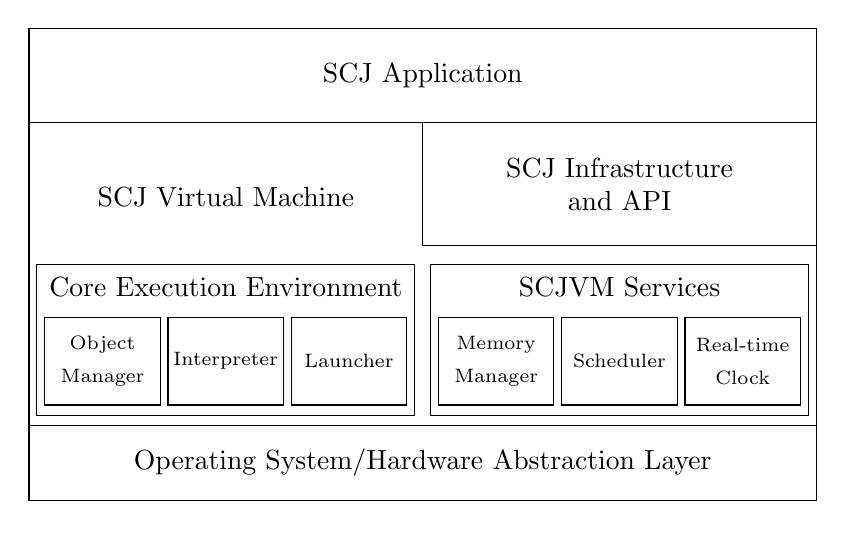
\begin{tikzpicture}
    \coordinate (width)  at (10cm,0cm);
    \coordinate (height) at (0cm,6cm);

    \path (0,0) -- (height)
    coordinate[pos=0.16] (OS boundary)
    coordinate[pos=0.18] (VM part bottom)
    coordinate[pos=0.50] (VM part top)
    coordinate[pos=0.54] (API boundary)
    coordinate[pos=0.80] (App boundary);

    \path (VM part bottom) -- (VM part top)
    coordinate[pos=0.65] (VM Service top)
    coordinate[pos=0.65] (CEE part top);

    \path (VM part bottom) -- (VM part top)
    coordinate[pos=0.85] (CEE ypos)
    coordinate[pos=0.85] (VM Services ypos);

    \path (0,0) -- (width)
    coordinate[pos=0.01] (CEE left)
    coordinate[pos=0.49] (CEE right)
    coordinate[pos=0.51] (VM Services left)
    coordinate[pos=0.99] (VM Services right)
    coordinate[pos=0.01] (CEE part sep)
    coordinate[pos=0.01] (VM Service sep);

    \path (CEE left) -- (CEE right)
    coordinate[pos=0.5] (CEE xpos);

    \path (VM Services left) -- (VM Services right)
    coordinate[pos=0.5] (VM Services xpos);

    \path (0,0) to node[pos=0.5] (mid) {} (width);
    \path (0,0) to node[pos=0.25] (quart) {} (width);

    \draw (0,0) rectangle (width |- height);

    \draw (OS boundary) -- ++(width);
    \path (0,0) rectangle node[pos=0.5] (OS) {} (width |- OS boundary);
    \draw (mid |- API boundary) rectangle node[pos=0.5] (API) {} (width |- App boundary);
    \draw (App boundary) -- ++(width);
    \path (App boundary) rectangle node[pos=0.5] (App) {} (width |- height);

    \path (quart |- API boundary) rectangle node[pos=0.4] (SCJVM) {} (quart |- App boundary);
    \draw[onslide=<2-3>{color=blue}, onslide=<4>{color=cyan}] (VM Services left |- VM part bottom) rectangle (VM Services right |- VM part top);
    \draw[onslide=<3-4>{color=red}, , onslide=<2>{color=blue}] (CEE left |- VM part bottom) rectangle (CEE right |- VM part top);
    \coordinate (CEE) at (CEE xpos |- CEE ypos);
    \coordinate (VM Services) at (VM Services xpos |- VM Services ypos);

    \node[align=center] at (App)   {SCJ Application};
    \node[align=center] at (API)   {SCJ Infrastructure\\and API};
    \node[align=center, onslide=<2-4>{color=blue}] at (SCJVM) {SCJ Virtual Machine};
    \node[align=center, onslide=<3-4>{color=red}, onslide=<2>{color=blue}] at (CEE)   {Core Execution Environment};
    \node[align=center, onslide=<2-3>{color=blue}, onslide=<4>{color=cyan}] at (VM Services)  {SCJVM Services};
    \node[align=center] at (OS)    {Operating System/Hardware Abstraction Layer};

    \foreach \x in {1,...,3}
    \pgfmathsetmacro{\a}{0.333*(\x - 1)}
    \pgfmathsetmacro{\b}{0.333*\x}
    \path ($(CEE left) + (VM part bottom)!0.07!(VM part top)$) --
    node[pos=\a] (CEE part \x start) {}
    node[pos=\b] (CEE part \x end) {}
    ($(CEE right) + (VM part bottom)!0.07!(VM part top) - (CEE part sep)$);

    \foreach \x in {1,...,3}
    \draw[onslide=<3-4>{color=red}, onslide=<2>{color=blue}] ($(CEE part \x start) + (CEE part sep)$)
    rectangle node[pos=0.5] (CEE part \x) {}
    (CEE part \x end |- CEE part top);

    \node[align=center, onslide=<3-4>{color=red}, onslide=<2>{color=blue}] at (CEE part 1) {\scriptsize Object \\ \scriptsize Manager};
    \node[align=center, onslide=<3-4>{color=red}, onslide=<2>{color=blue}] at (CEE part 2) {\scriptsize Interpreter};
    \node[align=center, onslide=<3-4>{color=red}, onslide=<2>{color=blue}] at (CEE part 3) {\scriptsize Launcher};

    \foreach \x in {1,...,3}
    \pgfmathsetmacro{\a}{0.333*(\x - 1)}
    \pgfmathsetmacro{\b}{0.333*\x}
    \path ($(VM Services left) + (VM part bottom)!0.07!(VM part top)$) --
    node[pos=\a] (VM Service \x start) {}
    node[pos=\b] (VM Service \x end) {}
    ($(VM Services right) + (VM part bottom)!0.07!(VM part top) - (VM Service sep)$);

    \foreach \x in {1,...,3}
    \draw[onslide=<4>{color=cyan}, onslide=<2-3>{color=blue}] ($(VM Service \x start) + (VM Service sep)$)
    rectangle node[pos=0.5] (VM Service \x) {}
    (VM Service \x end |- VM Service top);

    \node[align=center, onslide=<4>{color=cyan}, onslide=<2-3>{color=blue}] at (VM Service 1) {\scriptsize Memory \\ \scriptsize Manager};
    \node[align=center, onslide=<4>{color=cyan}, onslide=<2-3>{color=blue}] at (VM Service 2) {\scriptsize Scheduler};
    \node[align=center, onslide=<4>{color=cyan}, onslide=<2-3>{color=blue}] at (VM Service 3) {\scriptsize Real-time \\ \scriptsize Clock};
  \end{tikzpicture}
\end{frame}

\begin{frame}
  \frametitle{Overview of model}
  \begin{itemize}
  \item Core Execution Environment (CEE) has three components:
    \begin{itemize}
    \item Object Manager
      \begin{itemize}
      \item manages object representation and memory areas
      \end{itemize}
    \item Interpreter 
      \begin{itemize}
      \item handles execution of individual bytecodes
      \end{itemize}
    \item Launcher
      \begin{itemize}
      \item manages SCJVM startup and coordinates mission execution
      \end{itemize}
    \end{itemize}
  \item CEE parameters:
    \begin{itemize}
    \item Bytecode instructions ($bc$)
    \item Classes ($cs$)
    \item \texttt{Safelet} identifier ($sid$)
    \item Class initialisation order ($initOrder$)
    \end{itemize}
  \end{itemize}
  \vspace{-0.8cm}
  {\setlength{\zedindent}{2mm}
    \setlength{\zedleftsep}{2mm}
    \setlength{\zedtab}{0.7em}
    \begin{circus}
      \circprocess CEE(bc,cs,sid,initOrder) \circdef \\
      \t1 ObjMan(cs) \parallel Interpreter(bc,cs)  \parallel Launcher(sid,initOrder)
    \end{circus}}
\end{frame}

\begin{frame}
  \frametitle{Interpreter}
  \begin{itemize}
  \item Each thread is represented by a separate \Circus{} process.
  \item The state of each thread's process contains the program counter
    and frame stack.
  \item The Interpreter is a parallel composition of these threads.
  { \setlength{\zedindent}{0cm}
    \setlength{\zedleftsep}{0cm}
    \setlength{\abovedisplayskip}{0.1cm}
    \setlength{\belowdisplayskip}{0.1cm}
  \begin{circus}
    \circprocess Interpreter(bc,cs) \circdef \Parallel t : TID \setminus \{ idle \} \circspot Thr(bc, cs, t)
  \end{circus}}
  \item The thread processes proceed through a sequence of different
    actions as the scheduler starts and switches between them.
  \end{itemize}
  \centering
  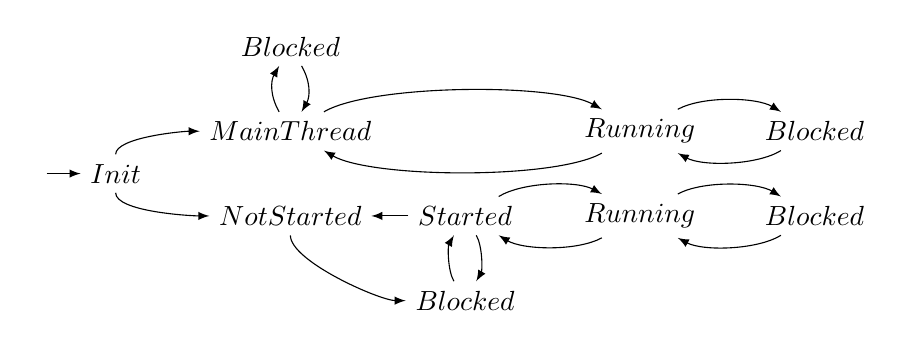
\begin{tikzpicture}
    \node at (9cm,0) (width) {};
    \node at (0,1.2cm) (height) {};

    \path (0,0) --
    node[pos=0.00] (Initxpos) {}
    node[pos=0.25] (MainThreadxpos) {}
    node[pos=0.25] (NotStartedxpos) {}
    node[pos=0.50] (Startedxpos) {}
    node[pos=0.75] (Runningxpos) {}
    node[pos=1.00] (Blockedxpos) {}
    (width);

    \path (0,0) --
    node[pos=-1]  (threadBlockedypos) {}
    node[pos=0]   (threadypos) {}
    node[pos=0.5] (Initypos) {}
    node[pos=1]   (mainypos) {}
    node[pos=2]   (mainBlockedypos) {}
    (height);

    \path (Initxpos |- Initypos) node (Init) {$Init$} ++(-1cm,0cm) node (start) {};
    \node at (MainThreadxpos |- mainypos) (IMn) {$MainThread$};
    \node at (Runningxpos |- mainypos) (MRn) {$Running$};
    \node at (MainThreadxpos |- mainBlockedypos) (MBl) {$Blocked$};
    \node at (Blockedxpos |- mainypos) (MB2) {$Blocked$};
    \node at (NotStartedxpos |- threadypos) (NSt) {$NotStarted$};
    \node at (Startedxpos |- threadypos) (Sta) {$Started$};
    \node at (Startedxpos |- threadBlockedypos) (TBl) {$Blocked$};
    \node at (Runningxpos |- threadypos) (TRn) {$Running$};
    \node at (Blockedxpos |- threadypos) (TB2) {$Blocked$};

    \draw[-latex] (start) to (Init);
    \draw[-latex] (Init) to[out=90,in=180,looseness=0.5] (IMn);
    \draw[-latex] (Init) to[out=270,in=180,looseness=0.5] (NSt);
    \draw[-latex] (IMn) to[bend left,looseness=0.5] (MRn);
    \draw[-latex] (MRn) to[bend left,looseness=0.5] (IMn);
    \draw[-latex] (MRn) to[bend left,looseness=0.7] (MB2);
    \draw[-latex] (MB2) to[bend left,looseness=0.7] (MRn);
    \draw[-latex] (IMn) to[bend left,looseness=1.0] (MBl);
    \draw[-latex] (MBl) to[bend left,looseness=1.0] (IMn);
    \draw[-latex] (NSt) to[out=270,in=180,looseness=0.5] (TBl);
    \draw[-latex] (TBl) to[bend left,looseness=0.7] (Sta);
    \draw[-latex] (Sta) to[bend left,looseness=0.7] (TBl);
    \draw[-latex] (Sta) to (NSt);
    \draw[-latex] (Sta) to[bend left,looseness=0.7] (TRn);
    \draw[-latex] (TRn) to[bend left,looseness=0.7] (Sta);
    \draw[-latex] (TB2) to[bend left,looseness=0.7] (TRn);
    \draw[-latex] (TRn) to[bend left,looseness=0.7] (TB2);
  \end{tikzpicture}
\end{frame}

\section{C Code}
\stepcounter{subsection}

\begin{frame}
  \frametitle{C Code Representation}
  \begin{itemize}
  \item The C code is represented by processes representing C threads.
  \item Each function is a separate action in the process.
  \item Function arguments are represented by action parameters.
  \item C variables are represented by \Circus{} variable blocks.
  \item \Circus{} recursion and conditionals represent C loops and conditionals.
  \item Objects are structs represented by Z schema bindings.
  \end{itemize}
\end{frame}

\section{Compilation Strategy}
\stepcounter{subsection}

\begin{frame}
  \frametitle{Overview of Compilation Strategy}
  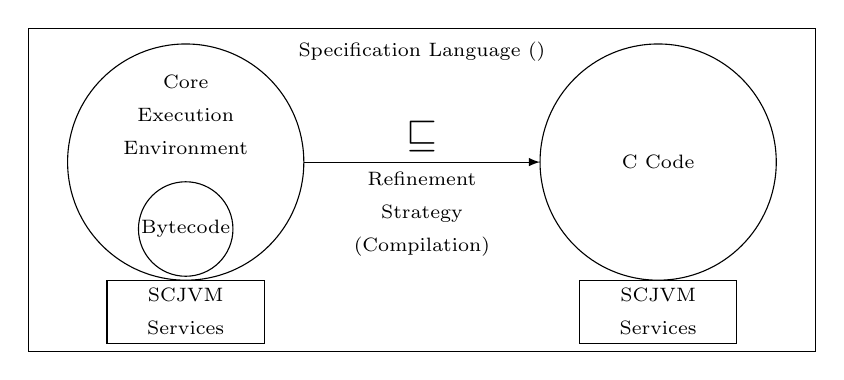
\begin{tikzpicture}
    \draw (0cm,0.4cm) rectangle (10cm,4.5cm);
    \draw (5cm,4.2cm) node[align=center] {\scriptsize Specification Language (\Circus{})};

    \draw (2cm,2.8cm)   circle[radius=1.5cm] ++(0cm,0.6cm) node[align=center] {\scriptsize Core\\\scriptsize Execution\\\scriptsize Environment};
    \draw (2cm,1.95cm)     circle[radius=0.6cm]               node[align=center] {\scriptsize Bytecode};
    \draw (8cm,2.8cm)   circle[radius=1.5cm]               node[align=center] {\scriptsize C Code};

    \draw (1cm,0.5cm) rectangle (3cm,1.3cm) node[pos=0.5,align=center] {\scriptsize SCJVM \\\scriptsize Services};
    \draw (7cm,0.5cm) rectangle (9cm,1.3cm) node[pos=0.5,align=center] {\scriptsize SCJVM \\\scriptsize Services};

    \path (3.5cm,2.8cm) edge[-latex]
    node[align=center, above] {\Large $\sqsubseteq$}
    node[align=center, below] {\scriptsize Refinement\\\scriptsize Strategy\\\scriptsize (Compilation)}
    (6.5cm,2.8cm);

    % \draw[-latex] (3cm,0.9cm) -- (7cm,0.9cm);
  \end{tikzpicture}
\end{frame}

\begin{frame}
  \frametitle{Overview of Compilation Strategy}
  \begin{itemize}
  \item Applies compilation rules to transform the interpreter.
  \item Divided into three stages:
    \begin{itemize}
    \item Elimination of Program Counter
    \item Elimination of Frame Stack
    \item Data Refinement of Memory
    \end{itemize}
  \end{itemize}
\end{frame}

\begin{frame}
  \frametitle{Example Program}
  \tiny
  \setlength{\zedleftsep}{0cm}
  \setlength{\zedindent}{0cm}
  \setlength{\zedtab}{0.3cm}
  \begin{columns}[c]
    \column{.3\textwidth}
    \begin{axdef}
      bc : ProgramAddress \pfun Bytecode
    \where
      programMemory = \{ \\
      \t1 0 \mapsto aload~0, \\
      \t1 1 \mapsto aload~1, \\
      \t1 2 \mapsto aload~2, \\
      \t1 3 \mapsto aload~3, \\
      \t1 4 \mapsto aload~4, \\
      \t1 5 \mapsto invokespecial~12, \\
      \t1 6 \mapsto aload~0, \\
      \t1 7 \mapsto aload~5, \\
      \t1 8 \mapsto putfield~15, \\
      \t1 9 \mapsto aload~0, \\
      \t1 10 \mapsto aload~6, \\
      \t1 11 \mapsto putfield~17, \\
      \t1 12 \mapsto return, \\
      \t1 13 \mapsto aload~0, \\
      \t1 14 \mapsto getfield~15, \\
      \t1 15 \mapsto invokevirtual~33, \\
      \t1 16 \mapsto astore~1, \\
      \t1 17 \mapsto aload~0, \\
      \t1 18 \mapsto getfield~17, \\
      \t1 19 \mapsto aload~1, \\
      \t1 20 \mapsto invokevirtual~39, \\
      \t1 21 \mapsto goto~4, \\
      \t1 22 \mapsto astore~1, \\
      \t1 23 \mapsto return \\
      \t1 \dots \\
      \} 
    \end{axdef}
    \column{.7\textwidth}
    \begin{axdef}
      InputHandler : Class
    \where
      InputHandler = \lblot \\
      \t1 constantPool == \{ \\
      \t2 1 \mapsto ClassRef~InputHandlerID, \\
      \t2 3 \mapsto ClassRef~PeriodicEventHandlerID, \\
      \t2 12 \mapsto MethodRef~(PeriodicEventHandlerID, PEHinit), \\
      \t2 15 \mapsto FieldRef~(InputHandlerID,input), \\
      \t2 17 \mapsto FieldRef~(InputHandlerID,buffer), \\
      \t2 33 \mapsto MethodRef(InputStreamID,read), \\
      \t2 34 \mapsto ClassRef~InputStreamID, \\
      \t2 39 \mapsto MethodRef~(BufferID,put), \\
      \t2 40 \mapsto ClassRef~BufferID \\
      \t1 \}, \\
      \t1 this == 1, \\
      \t1 super == 3, \\
      \t1 interfaces == \{\}, \\
      \t1 methodEntry == \{ init \mapsto 0, handleAsyncEvent \mapsto 13 \}, \\
      \t1 methodEnd == \{ init \mapsto 12, handleAsyncEvent \mapsto 23 \}, \\
      \t1 methodLocals == \{ init \mapsto 7, handleAsyncEvent \mapsto 2 \}, \\
      \t1 methodStackSize == \{ init \mapsto 5, handleAsyncEvent \mapsto 2 \}, \\
      \t1 fields == \{ input, buffer \}, \\
      \t1 staticFields == \{\} \\
      \rblot
    \end{axdef}
    \vspace{-0.5cm}
    \begin{axdef}
      cs : ClassID \pfun Class
    \where
      cs = \{ InputHandlerID \mapsto InputHandler, \dots \}
    \end{axdef}
  \end{columns}
\end{frame}

\begin{frame}
  \frametitle{Elimination of Program Counter}
  \begin{itemize}
  \item Operates on the $Thr$ processes of the interpreter
  \item Introduces the control flow constructs of the C code.
  \item Copies methods into separate actions.
  \item Removes program counter from state.
  \end{itemize}
\end{frame}

\begin{frame}
  \frametitle{Elimination of Program Counter}
  \begin{algorithm}[H]
    \begin{algorithmic}[1]
      \State \Call{ExpandBytecode}{}
      \State \Call{IntroduceSequentialComposition}{}
      \While{$\lnot$\Call{AllMethodsSeparated}{}}
      \State \Call{IntroduceLoopsAndConditionals}{}
      \State \Call{SeparateCompleteMethods}{}
      \State \Call{ResolveMethodCalls}{}
      \EndWhile
      \State \Call{RefineMainActions}{}
      \State \Call{RemovePCFromState}{}
    \end{algorithmic}
    \caption{Elimination of Program Counter}
  \end{algorithm}
\end{frame}

\begin{frame}
  \frametitle{Elimination of Program Counter}
  \centering
  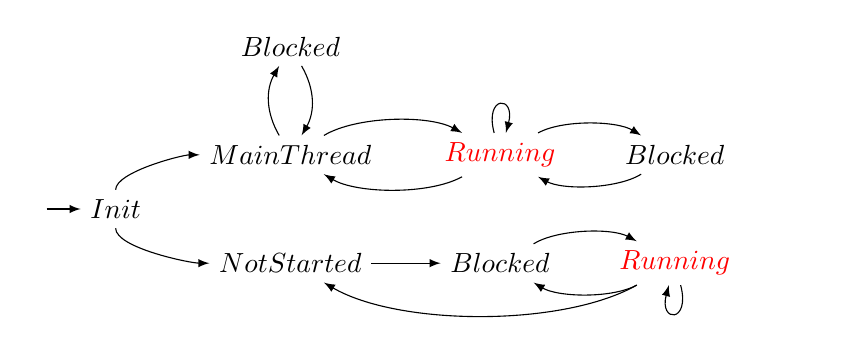
\begin{tikzpicture}
    \node at (9cm,0) (width) {};
    \node at (0,1.5cm) (height) {};

    \path (0,0) --
    node[pos=0.00] (Initxpos) {}
    node[pos=0.25] (Interpreterxpos) {}
    node[pos=0.55] (Executexpos) {}
    node[pos=0.8] (ExecuteAndPollxpos) {}
    (width);

    \path (0,0) --
    node[pos=0] (threadypos) {}
    node[pos=0.5] (Initypos) {}
    node[pos=1] (mainypos) {}
    node[pos=2] (mainBlockedypos) {}
    (height);

    \path (Initxpos |- Initypos) node (Init) {$Init$} ++(-1cm,0cm) node (start) {};
    \node at (Interpreterxpos |- mainypos) (IMn) {$MainThread$};
    \node at (Executexpos |- mainypos) (MRn) {\color{red} $Running$};
    \node at (Interpreterxpos |- mainBlockedypos) (MBl) {$Blocked$};
    \node at (ExecuteAndPollxpos |- mainypos) (MB2) {$Blocked$};
    \node at (Interpreterxpos |- threadypos) (NSt) {$NotStarted$};
    \node at (Executexpos |- threadypos) (TBl) {$Blocked$};
    \node at (ExecuteAndPollxpos |- threadypos) (TRn) {\color{red} $Running$};

    \draw[-latex] (start) to (Init);
    \draw[-latex] (Init) to[out=90,in=180,looseness=0.5] (IMn);
    \draw[-latex] (Init) to[out=270,in=180,looseness=0.5] (NSt);
    \draw[-latex] (IMn) to[bend left,looseness=0.7] (MRn);
    \draw[-latex] (MRn) to[bend left,looseness=0.7] (IMn);
    \draw[-latex] (MRn) to[bend left,looseness=0.7] (MB2);
    \draw[-latex] (MB2) to[bend left,looseness=0.7] (MRn);
    \draw[-latex] (IMn) to[bend left,looseness=1.0] (MBl);
    \draw[-latex] (MBl) to[bend left,looseness=1.0] (IMn);
    \draw[-latex] (NSt) to (TBl);
    \draw[-latex] (TBl) to[bend left,looseness=0.7] (TRn);
    \draw[-latex] (TRn) to[bend left,looseness=0.7] (TBl);
    \draw[-latex] (TRn) to[bend left,looseness=0.7] (NSt);
    \draw[-latex] (TRn) to[loop below] (TRn);
    \draw[-latex] (MRn) to[loop above] (MRn);
  \end{tikzpicture}
\end{frame}

\begin{frame}
  \frametitle{Elimination of Program Counter}
  \tiny
  \begin{circus}
    Running \circdef \\
    \t1 \circif frameStack = \emptyset \circthen \Skip \\
    \t1 {} \circelse frameStack \neq \emptyset \circthen {} \\
    \t2 {} \circif pc = 0 \circthen HandleAload(0) \circseq pc := 1 \\
    \t2 {} \circelse pc = 1 \circthen HandleAload(1) \circseq pc := 2 \\
    \t2 {} \circelse pc = 2 \circthen HandleAload(2) \circseq pc := 3 \\
    \t2 {} \circelse pc = 3 \circthen HandleAload(3) \circseq pc := 4 \\
    \t2 {} \circelse pc = 4 \circthen HandleAload(4) \circseq pc := 5 \\
    \t2 {} \circelse pc = 5 \circthen HandleInvokespecial(12) \\
    \t2 {} \circelse pc = 6 \circthen HandleAload(0) \circseq pc := 7 \\
    \t2 {} \circelse pc = 7 \circthen HandleAload(5) \circseq pc := 8 \\
    \t2 {} \circelse pc = 8 \circthen HandlePutfield(15) \circseq pc := 9 \\
    \t2 {} \circelse pc = 9 \circthen HandleAload(0) \circseq pc := 10 \\
    \t2 {} \circelse pc = 10 \circthen HandleAload(6) \circseq pc := 11 \\
    \t2 {} \circelse pc = 11 \circthen HandlePutfield(17) \circseq pc := 12 \\
    \t2 {} \circelse pc = 12 \circthen HandleReturn \\
    \t2 {} \circelse pc = 13 \circthen HandleAload(0) \circseq pc := 14 \\
    \t2 {} \circelse pc = 14 \circthen HandleGetfield(15) \circseq pc := 15 \\
    \t2 {} \circelse pc = 15 \circthen HandleInvokevirtual(33) \\
    \t2 {} \circelse pc = 16 \circthen HandleAstore(1) \circseq pc := 17 \\
    \t2 {} \circelse pc = 17 \circthen HandleAload(0) \circseq pc := 18 \\
    \t2 {} \circelse pc = 18 \circthen HandleGetfield(17) \circseq pc := 19 \\
    \t2 {} \circelse pc = 19 \circthen HandleAload(1) \circseq pc := 20 \\
    \t2 {} \circelse pc = 20 \circthen HandleInvokevirtual(39) \\
    \t2 {} \circelse pc = 21 \circthen pc := 23 \\
    \t2 {} \circelse pc = 22 \circthen HandleAstore(1) \circseq pc := 23 \\
    \t2 {} \circelse pc = 23 \circthen HandleReturn \\
    \t2 \dots \\
    \t2 {} \circfi \circseq Poll \circseq Running \\
    \t1 \circfi
  \end{circus}
\end{frame}

\begin{frame}
  \frametitle{Elimination of Program Counter}
  \small
  \begin{rul}[Sequence introduction]
    \label{sequence-introduction-rule}
    \setlength{\zedindent}{0cm}
    \setlength{\zedtab}{0.5cm}
    \setlength{\abovedisplayskip}{0.1cm}
    \setlength{\belowdisplayskip}{0.1cm}
    If $i \neq j$ and
    \begin{circus}
      \{frameStack \neq \emptyset\} \circseq A {} \quad = \quad 
      \{frameStack \neq \emptyset\} \circseq A \circseq \{frameStack \neq \emptyset\}
    \end{circus}
    then,
    \begin{circus}
      \begin{array}{l}
        \circmu X \circspot \\
        \t1  \circif frameStack = \emptyset \circthen \Skip \\
        \t1  {} \circelse frameStack \neq \emptyset \circthen {} \\
        \t2 \circif {} \cdots {} \\
        \t2 {} \circelse pc = i \circthen \\
        \t3 A \circseq pc := j \\
        \t2 {} \circelse pc = j \circthen B \\
        \t2 {} \cdots {} \\
        \t2 \circfi \circseq Poll \circseq X \\
        \t1 \circfi
      \end{array}
      \circrefines_A
      \begin{array}{l}
        \circmu X \circspot \\
        \t1 \circif frameStack = \emptyset \circthen \Skip \\
        \t1 {} \circelse frameStack \neq \emptyset \circthen {} \\
        \t2 \circif {} \cdots {} \\
        \t2 {} \circelse pc = i \circthen {} \\
        \t3 A \circseq pc := j \circseq Poll \circseq B \\
        \t2 {} \circelse pc = j \circthen B \\
        \t2 {} \cdots {} \\
        \t2 \circfi \circseq Poll \circseq X \\
        \t1 \circfi
      \end{array}
    \end{circus}
  \end{rul}
\end{frame}

\begin{frame}
  \frametitle{Elimination of Program Counter}
  \centering
  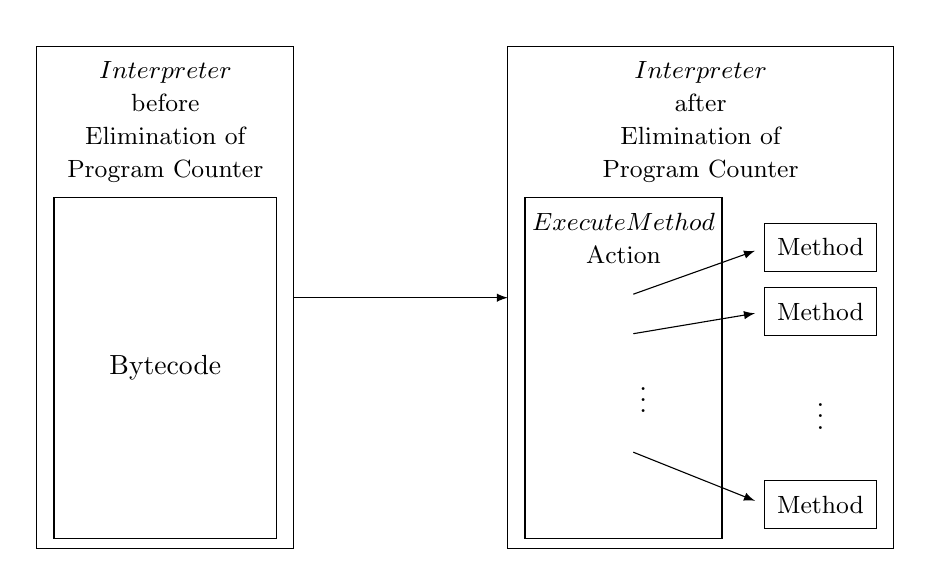
\begin{tikzpicture}
    \node at (11cm,0) (width) {};
    \node at (0,6.5cm) (height) {};

    \path (0,0) --
    node[pos=0.00] (Interpreter1Left) {}
    node[pos=0.02] (BytecodeLeft) {}
    node[pos=0.28] (BytecodeRight) {}
    node[pos=0.30] (Interpreter1Right) {}
    node[pos=0.50] (CenterXPos) {}
    node[pos=0.55] (Interpreter2Left) {}
    node[pos=0.57] (ExecuteMethodLeft) {}
    node[pos=0.685] (ExecuteMethodAnchorsXPos) {}
    node[pos=0.80] (ExecuteMethodRight) {}
    node[pos=0.85] (MethodsLeft) {}
    node[pos=0.98] (MethodsRight) {}
    node[pos=1.00] (Interpreter2Right) {}
    (width);

    \path (0,0) --
    node[pos=0.00] (InterpreterBot) {}
    node[pos=0.02] (ContentsBot) {}
    node[pos=0.20] (ExecuteMethodAnchorsBot) {}
    node[pos=0.50] (CenterYPos) {}
    node[pos=0.50] (ExecuteMethodAnchorsTop) {}
    node[pos=0.70] (ContentsTop) {}
    node[pos=1.00] (InterpreterTop) {}
    (height);

    \draw (Interpreter1Left |- InterpreterBot) rectangle
    (Interpreter1Right |- InterpreterTop);
    \draw (Interpreter2Left |- InterpreterBot) rectangle
    (Interpreter2Right |- InterpreterTop);

    \draw (BytecodeLeft |- ContentsBot) rectangle
    node[pos=0.5,align=center] {Bytecode}
    (BytecodeRight |- ContentsTop);
    \draw (ExecuteMethodLeft |- ContentsBot) rectangle
    (ExecuteMethodRight |- ContentsTop);    
    \path (ExecuteMethodAnchorsXPos |- ContentsBot) --
    node[pos=0.88,align=center] {\small $ExecuteMethod$\\\small Action}
    (ExecuteMethodAnchorsXPos |- ContentsTop);
    
    \path (Interpreter1Left |- ContentsTop) rectangle
    node[pos=0.5,align=center] {\small $Interpreter$\\\small before\\\small Elimination of\\\small Program Counter}
    (Interpreter1Right |- InterpreterTop);
    \path (Interpreter2Left |- ContentsTop) rectangle
    node[pos=0.5,align=center] {\small $Interpreter$\\\small after\\\small Elimination of\\\small Program Counter}
    (Interpreter2Right |- InterpreterTop);
    
    \foreach \x in {1,...,5}
    \pgfmathsetmacro{\a}{0.2*(\x - 1)}
    \pgfmathsetmacro{\b}{0.2*(\x - 1) + 0.15}
    \path (ContentsBot) --
    node[pos=\a] (Method\x Bot) {}
    node[pos=\b] (Method\x Top) {}
    (ContentsTop);

    \foreach \x in {1,...,5}
    \path (MethodsLeft |- Method\x Bot) --
    node[pos=0.5] (Method\x Anchor) {}
    (MethodsLeft |- Method\x Top);

    \foreach \x in {1,...,5}
    \pgfmathsetmacro{\a}{0.25*(\x - 1)}
    \path (ExecuteMethodAnchorsXPos |- ExecuteMethodAnchorsBot) --
    node[pos=\a] (ExecuteMethodAnchor\x ) {}
    (ExecuteMethodAnchorsXPos |- ExecuteMethodAnchorsTop);
    
    \draw (MethodsLeft |- Method1Bot) rectangle
    node[pos=0.5] {\small Method}
    (MethodsRight |- Method1Top);
    \draw (MethodsLeft |- Method4Bot) rectangle
    node[pos=0.5] {\small Method}
    (MethodsRight |- Method4Top);
    \draw (MethodsLeft |- Method5Bot) rectangle
    node[pos=0.5] {\small Method}
    (MethodsRight |- Method5Top);
    \path (MethodsLeft |- Method2Bot) rectangle
    node[pos=0.5,align=center] {\vdots}
    (MethodsRight |- Method3Top);

    \draw[-latex] (ExecuteMethodAnchor1) -- (Method1Anchor);
    \draw[-latex] (ExecuteMethodAnchor4) -- (Method4Anchor);
    \draw[-latex] (ExecuteMethodAnchor5) -- (Method5Anchor);
    \path (ExecuteMethodAnchor2) --
    node[pos=0.5,align=center] {\hspace{0.5cm}\vdots}
    (ExecuteMethodAnchor3);

    \draw[-latex] (Interpreter1Right |- CenterYPos) --
    node[above] {\huge $\circrefines$}
    (Interpreter2Left |- CenterYPos);
  \end{tikzpicture}
\end{frame}

\begin{frame}[shrink]
  \frametitle{Elimination of Program Counter}
  \setlength{\zedleftsep}{0cm}
  \setlength{\zedindent}{0cm}
  \begin{circus}
    InputHandler\_Init \circdef HandleAload(0) \circseq Poll \circseq HandleAload(1) \circseq \\
    \t1 Poll \circseq HandleAload(2) \circseq Poll \circseq HandleAload(3) \circseq Poll \circseq \\
    \t1 HandleAload(4) \circseq Poll \circseq HandleInvokespecial(12) \circseq Poll \circseq \\
    \t1 PeriodicEventHandler\_Init \circseq Poll \circseq HandleAload(0) \circseq Poll \circseq \\
    \t1 HandleAload(5) \circseq Poll \circseq HandlePutfield(15) \circseq Poll \circseq \\
    \t1 HandleAload(0) \circseq Poll \circseq HandleAload(6) \circseq Poll \circseq \\
    \t1 HandlePutfield(17) \circseq Poll \circseq HandleReturn
  \end{circus}
  \begin{circus}
    InputHandler\_HandleAsyncEvent \circdef HandleAload(0) \circseq Poll \circseq \\
    \t1 HandleGetfield(15) \circseq Poll \circseq HandleInvokevirtual(33) \circseq Poll \circseq \\
    \t1 InputStream\_Read \circseq Poll \circseq HandleAstore(1) \circseq Poll \circseq \\
    \t1 HandleAload(0) \circseq Poll \circseq HandleGetfield(17) \circseq Poll \circseq \\
    \t1 HandleAload(1) \circseq Poll \circseq HandleInvokevirtual(39) \circseq Poll \circseq \\
    \t1 Buffer\_Put \circseq Poll \circseq Poll \circseq HandleReturn
  \end{circus}
\end{frame}

\begin{frame}
  \frametitle{Elimination of Frame Stack}
  \begin{itemize}
  \item Introduces variables and parameters representing Java local
    variables and operand stack slots.
  \item Removes the frame stack from the state, copying its
    information to the introduced variables.
  \end{itemize}
\end{frame}

\begin{frame}[shrink]
  \frametitle{Elimination of Frame Stack}
  \setlength{\zedleftsep}{0cm}
  \setlength{\zedindent}{0cm}
  \begin{circus}
    InputHandler\_Init \circdef \circval var0, var1, var2, var3, var4, var5, var6 : Word  \circspot \\
    \t1 \circvar stack0, stack1, stack2, stack3, stack4 : Word \circspot \\
    \t1 stack0 := var0 \circseq Poll \circseq stack1 := var1 \circseq Poll \circseq stack2 := var2 \circseq \\
    \t1 Poll \circseq stack3 := var3 \circseq Poll \circseq stack4 := var4 \circseq Poll \circseq Poll \\
    \t1 PeriodicEventHandler\_Init(stack0, stack1, stack2, stack3, stack4) \circseq \\
    \t1 stack0 := var0 \circseq Poll \circseq stack1 := var5 \circseq Poll \circseq \\
    \t1 putField!stack0!input!stack1 \then \Skip \circseq Poll \circseq stack0 := var0 \circseq \\
    \t1 Poll \circseq stack1 := var6 \circseq Poll \circseq \\
    \t1 putField!stack0!buffer!stack1 \then \Skip \circseq Poll
  \end{circus}
  \begin{circus}
    InputHandler\_HandleAsyncEvent \circdef \circval var0 : Word \circspot \\
    \t1 \circvar var1, stack0, stack1 : Word \circspot stack0 := var0 \circseq Poll \circseq \\
    \t1 getField!stack0!input \then getFieldRet?value \then stack0 := value \circseq \\
    \t1 Poll \circseq Poll \circseq InputStream\_Read(stack0, stack0) \circseq Poll \circseq var1 := stack0 \circseq \\
    \t1 Poll \circseq stack0 := var0 \circseq Poll \circseq \\
    \t1 getField!stack0!buffer \then getFieldRet?value \then stack0 := value \circseq \\
    \t1 Poll \circseq stack1 := var1 \circseq Poll \circseq Poll \circseq Buffer\_Put(stack0, stack1) \circseq \\
    \t1 Poll \circseq Poll
  \end{circus}
\end{frame}

\begin{frame}
  \frametitle{Data Refinement of Memory}
  \begin{itemize}
  \item Creates types for structs representing objects.
  \item Refines the Object Manager to use the new types.
  \item Refines the Interpreter to access objects via the new types.
  \end{itemize}
\end{frame}

\begin{frame}[shrink]
  \frametitle{Data Refinement of Memory}
  \setlength{\zedleftsep}{0cm}
  \setlength{\zedindent}{0cm}
  \begin{circus}
    InputHandler\_Init \circdef \circval var0, var1, var2, var3, var4, var5, var6 : Word  \circspot \\
    \t1 \circvar stack0, stack1, stack2, stack3, stack4 : Word \circspot \\
    \t1 stack0 := var0 \circseq Poll \circseq stack1 := var1 \circseq Poll \circseq stack2 := var2 \circseq Poll \circseq \\
    \t1 stack3 := var3 \circseq Poll \circseq stack4 := var4 \circseq Poll \circseq Poll \circseq \\
    \t1 PeriodicEventHandler\_Init(stack0, stack1, stack2, stack3, stack4) \circseq \\
    \t1 stack0 := var0 \circseq Poll \circseq stack1 := var5 \circseq Poll \circseq \\
    \t1 {\color{red} getObject?stack0 \then getObjectRet?struct \then {}} \\
    \t1 {\color{red} putObject!stack0!(updateInputHandler\_input~struct~stack1)  \then {}  \Skip} \circseq \\
    \t1 Poll \circseq stack0 := var0 \circseq Poll \circseq stack1 := var6 \circseq Poll \circseq \\
    \t1 {\color{red} getObject?stack0 \then getObjectRet?struct \then {}} \\
    \t1 {\color{red} putObject!stack0!(updateInputHandler\_buffer~struct~stack1) \then \Skip} \circseq Poll
  \end{circus}
  \begin{circus}
    InputHandler\_HandleAsyncEvent \circdef \circval var0 : Word \circspot \\
    \t1 \circvar var1, stack0, stack1 : Word \circspot \\
    \t1 stack0 := var0 \circseq Poll \circseq {\color{red} getObject!stack0 \then getObjectRet?struct \then {}} \\
    \t1 {\color{red} stack0 := (castInputHandler~struct).input} \circseq Poll \circseq Poll \circseq \\
    \t1 InputStream\_Read(stack0, stack0) \circseq Poll \circseq var1 := stack0 \circseq \\
    \t1 Poll \circseq stack0 := var0 \circseq Poll \circseq {\color{red} getObject!stack0 \then {}} \\
    \t1 {\color{red} getObjectRet?struct \then stack0 := (castInputHandler~struct).buffer} \circseq \\
    \t1 Poll \circseq stack1 := var1 \circseq Poll \circseq Poll \circseq Buffer\_Put(stack0, stack1) \circseq Poll \circseq Poll
  \end{circus}
\end{frame}

\begin{frame}[fragile,shrink]
  \frametitle{C code}
\begin{lstlisting}
void InputHandler_init(uint32_t var0, var1, var2, var3, var4, var5, var6) {
  uint32_t stack0, stack1, stack2, stack3, stack4;
  stack0 = var0;
  stack1 = var1;
  stack2 = var2;
  stack3 = var3;
  stack4 = var4;
  PeriodicEventHandler_init(stack0, stack1,stack2, stack3, stack4);
  stack0 = var0;
  stack1 = var5;
  ((InputHandler *) stack0)->input = stack1;
  stack0 = var0;
  stack1 = var6;
  ((InputHandler *) stack0)->buffer = stack1;
  return;
}
\end{lstlisting}
\begin{lstlisting}
void InputHandler_handleAsyncEvent(uint32_t var0) {
  uint32_t var1, stack0, stack1;
  stack0 = var0;
  stack0 = ((InputHandler *) stack0)->input;
  stack0 = InputStream_read(stack0);
  var1 = stack0;
  stack0 = var0;
  stack0 = ((InputHandler *) stack0)->buffer;
  stack1 = var1;
  Buffer_put(stack0,stack1);
  return;
}
\end{lstlisting}
\end{frame}


\section{Conclusion}
\stepcounter{subsection}

\begin{frame}
  \frametitle{Conclusion}
  \begin{itemize}
  \item Correct execution of an SCJ program requires a correct VM.
  \item There is not yet a formally verified VM.
  \item We provide a formal model of SCJ interpreter that can be
    used as the basis for a formally verified VM.
  \item We also provide a compilation strategy for applying provable
    compilation rules that can be used to transform an SCJ bytecode
    program into equivalent C code.
  \end{itemize}
\end{frame}


\end{document}